\section{Data Description and Preprocessing}

\subsection{Data description}
As previously described in detail, the main dataset contains \(7{,}773\) labeled tracks and \(192\) columns in total: \(191\) acoustic descriptors and the response variable \texttt{GENRE}. The five musical genres represented in the study are \textit{Blues} with \(1{,}074\) tracks, \textit{Classical} with \(2{,}318\) tracks, \textit{Jazz} with \(2{,}036\) tracks, \textit{Pop} with \(1{,}033\) tracks, and \textit{Rock} with \(1{,}312\) tracks. This class distribution is summarized in Fig.~\ref{fig:genre-proportions}.

The companion holdout file contains \(3{,}798\) additional tracks with the same \(191\) predictors, but without genre labels.

\begin{figure}[!t]
\centering
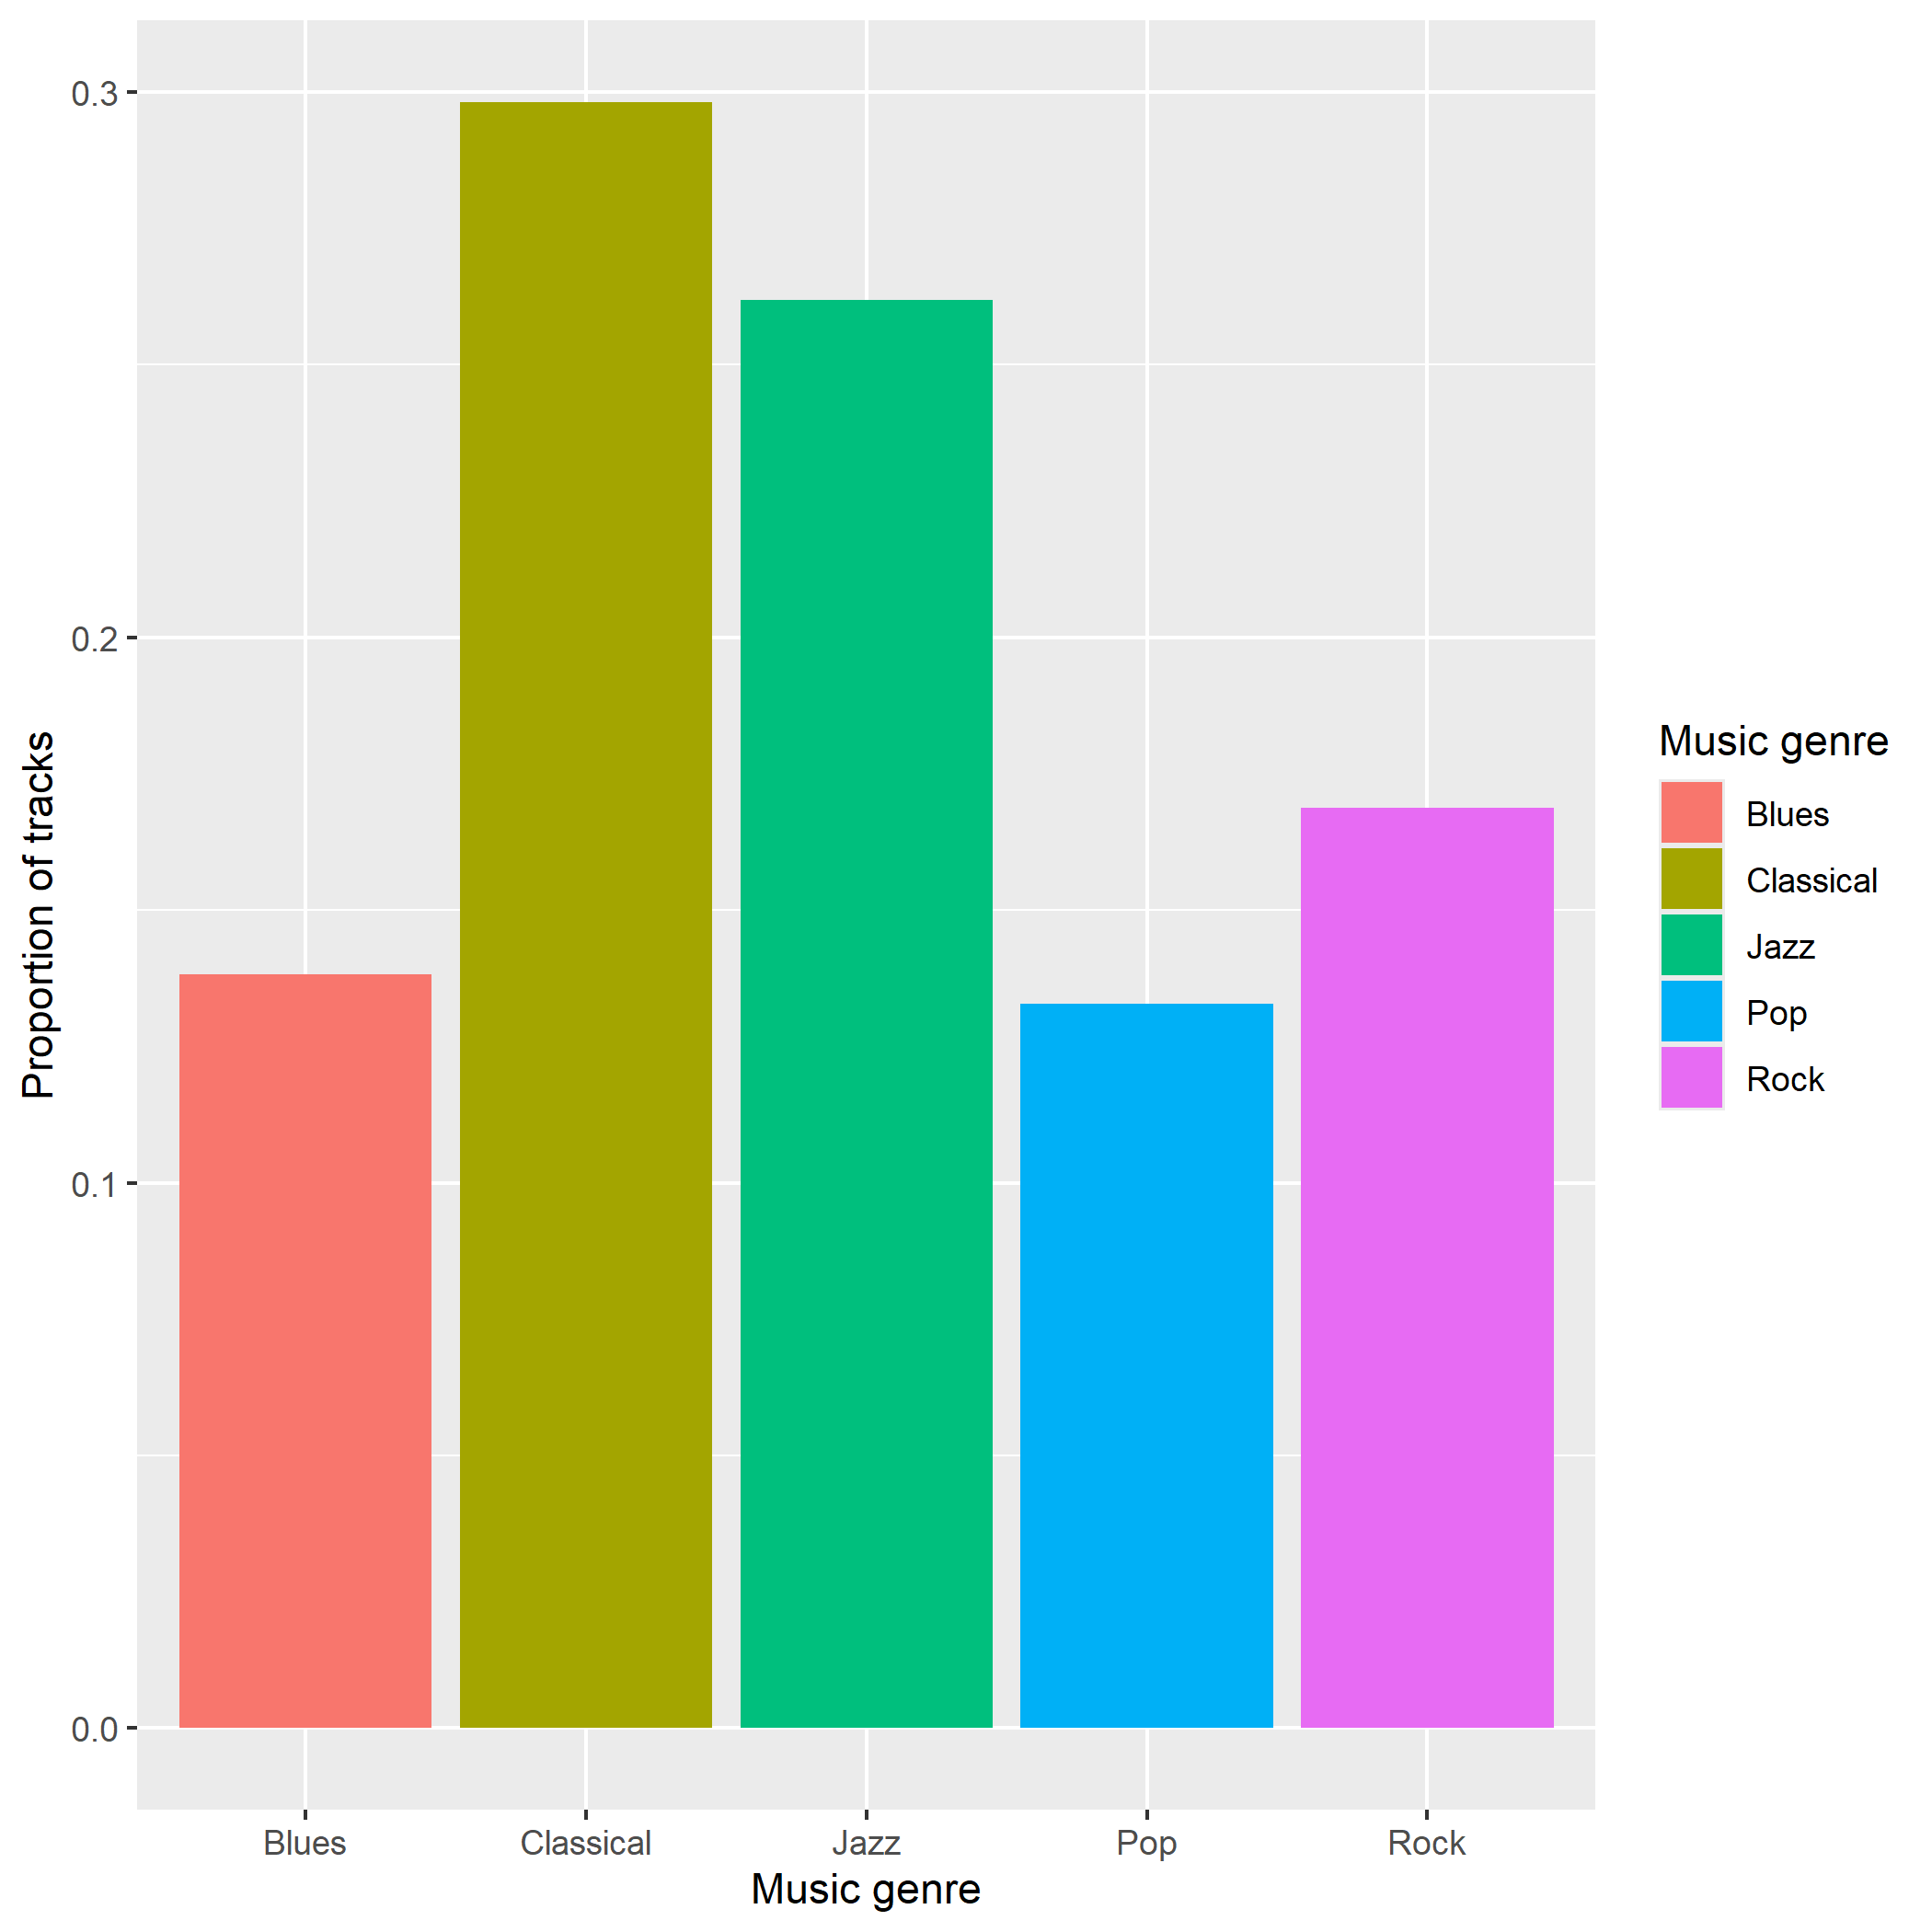
\includegraphics[width=0.78\columnwidth]{../output/part1/genre_proportions.png}
\caption{Observed proportions of the five genres in the labeled dataset. Classical and Jazz are the two most represented classes.}
\label{fig:genre-proportions}
\end{figure}

The dataset contains no missing values. The 191 numerical predictors are grouped into several families of acoustic descriptors, including MPEG-7-based spectral features, audio spectrum envelope summaries, spectral flatness measures, MFCC coefficients, and dedicated time-domain descriptors related to RMS energy, threshold crossings, and zero-crossing behavior.

\subsection{Data Preprocessing}

\cite{vandenberg2006preprocessing} discusses the possibility of applying a logarithmic transformation when large differences in scale are observed among variables characterized by strong asymmetry. This transformation is useful because it reduces large values more strongly than small values, which helps stabilize dispersion and prevents the analysis from being dominated by variables with higher magnitudes.

In order to identify the variables in the database that satisfy these dispersion-related conditions and may therefore benefit from the application of a logarithmic transformation, several complementary analyses are proposed. First, the mean-to-median ratio is computed as a simple descriptive indicator of asymmetry. For a roughly symmetric variable, the mean and the median are expected to be close, so the ratio should be near \(1\). A ratio clearly larger than \(1\) suggests right-skewness, since a small number of large observations pulls the mean upward relative to the median.The corresponding results are shown in the supplementary figure \ref{fig:mean_ratio}.

This analysis is further complemented by the introduction of a skewness estimate, defined as the third central moment of each variable. This measure provides a more detailed characterization of the asymmetry of the corresponding distribution. Large positive skewness values indicate the presence of a long right tail, whereas values close to zero are associated with a more symmetric distribution. The mathematical definition of skewness is presented in Appendix~\ref{app:skewness}, specifically in Equation~\eqref{eq:skewness}. In addition, Fig.~\ref{fig:skewness_candidates} shows the main candidate variables for the application of a logarithmic transformation according to their skewness values.

As a final complementary diagnostic, we examine heteroscedasticity in the conceptual sense of a \emph{spread-versus-level} pattern, that is, a situation in which the dispersion of a variable tends to increase with its magnitude instead of remaining approximately stable. This criterion is relevant here because a logarithmic transformation is especially useful when large values are not only more frequent in the tail, but also more variable. For that reason, an empirical heteroscedasticity score is used together with the mean-to-median ratio and the skewness coefficient to identify plausible candidates for logarithmic transformation. The complete definition of this score and its theoretical motivation are given in Appendix~\ref{app:skewness}, Subsection~\ref{subsec:heteroscedasticity}; the corresponding ranking of variables is displayed in Fig.~\ref{fig:heteroscedasticity_candidates}.

Nevertheless, before applying the transformation, it is important to consider the observation made by \cite{feng2014log} regarding the logarithmic transformation: it does not necessarily guarantee symmetry. The improvement in terms of asymmetry reduction, approximation to normality, and variance stabilization is favored when the original data distribution is close to a log-normal distribution. For this reason, in order to assess whether a candidate variable can be reasonably considered approximately log-normal, a Shapiro--Wilk normality test is applied to its logarithmic transformation, considering only variables with strictly positive values. This criterion is based on the fact that, if a variable \(X\) follows a log-normal distribution, then \(\log(X)\) should approximately follow a normal distribution. The common candidate set is listed in Appendix~\ref{app:skewness}, Subsection~\ref{subsec:log_normality}, Table~\ref{tab:common_candidates}, while the corresponding Shapiro--Wilk rankings are reported in Fig.~\ref{fig:log_normality_candidates} and Table~\ref{tab:log_normality_candidates}.

Considering the 30 variables showing the strongest suitability as candidates for the application of a logarithmic transformation, the variables \texttt{PAR\_SC\_V} and \texttt{PAR\_ASC\_V} are common to the lists of the 30 best candidates according to the previously described criteria; see Appendix~\ref{app:skewness}, Table~\ref{tab:common_candidates}. After applying the Shapiro--Wilk normality test to the logarithmically transformed variables, \texttt{PAR\_SC\_V} is found to be the variable that best follows the desired distributional behavior, in accordance with the recommendations of \cite{feng2014log}; this ranking is summarized in Fig.~\ref{fig:log_normality_candidates} and Table~\ref{tab:log_normality_candidates}. This makes \texttt{PAR\_SC\_V} the strongest candidate for the application of the logarithmic transformation. Additionally, \texttt{PAR\_ASC\_V} appears consistently among the variables of interest and is also included among the variables for which the Shapiro--Wilk test suggests a distribution more compatible with obtaining favorable results after the logarithmic transformation. Therefore, as part of the preprocessing stage and before centering and scaling the data, the logarithmic transformation is applied to \texttt{PAR\_SC\_V}, which is the strongest candidate. In addition, \texttt{PAR\_ASC\_V} is also included as a weaker but still relevant candidate, since its empirical distribution remains suitable for the application of this transformation. Consequently, both transformations are applied to the training data.


From the multivariate analysis, the inspection of the correlation matrix among the variables in the dataset reveals a second important preprocessing issue: redundancy.

A total of 22 variable pairs with absolute correlation greater than \(0.99\) are detected. Among them, 20 correspond to exact duplicates of the form \((\texttt{PAR\_MFCC}j, \texttt{PAR\_MFCCV}j)\), for \(j = 1, \ldots, 20\). This result is consistent with the duplicated block reported in variables 148 to 167 of the project statement.

The two remaining highly correlated pairs are \((\texttt{PAR\_ZCD}, \texttt{PAR\_ZCD\_10FR\_MEAN})\), with a correlation of \(0.9958\), and \((\texttt{PAR\_1RMS\_TCD}, \texttt{PAR\_1RMS\_TCD\_10FR\_MEAN})\), with a correlation of \(0.9938\). To reduce redundancy and avoid introducing duplicated information into the subsequent analyses, one representative variable is retained from each pair, while the corresponding redundant companion variable is removed.

The group of descriptor variables \texttt{PAR\_ASE\_M}, \texttt{PAR\_ASE\_MV}, \texttt{PAR\_SFM\_M}, and \texttt{PAR\_SFM\_MV} is also removed. These variables are computed as averages over families of variables that are already included in the dataset. Therefore, retaining both the detailed band-level variables and their aggregated summaries would introduce strong collinearity into the predictor space. This redundancy could make model estimation less stable, complicate the interpretation of the results, and lead to artificial overrepresentation of descriptor families that are already accounted for by their individual components. For this reason, these aggregated variables are excluded from the subsequent analyses. After all filtering steps, the predictor space is reduced from \(191\) to \(165\) variables.